\DiaryEntry{Subgroups}{2023-07-11}{Algebra}

A subgroup $H$ is a non-empty subset of a group $G$ which satisfies the same axioms as the group. More formally, we have the following definition.

\begin{definition}
A subgroup $H$ of a group $G$ is a non-empty set which is closed under multiplication and inverses; ie $x, y \in H$ implies $x \cdot y \in H$ and $x^{-1} \in H$. We shall write $H \leq G$ for the subgroup $H$.
\end{definition}

As an example, we have the set of even integers being a subgroup of the integers (under addition).

Checking whether a set is a subgroup can be done by checking above definition for all elements $x, y \in H$. However, we can simplify this somewhat.

\begin{theorem}
A subset $H$ of a group $G$ is a subgroup iff $H \neq \{\}$ and for all $x, y \in H, xy^{-1} \in H$.
\end{theorem}

\subsection{Centralizers, Normalizers, Stabilizers, and Kernels}

We next introduce several families of subgroups of an arbitrary group $G$ which provide many examples of subgroups. In the following, let $A$ be a non-empty subset of $G$.

\begin{definition}
The \emph{centralizer} $C_G(A)$ of $A$ in $G$ is defined as $C_G(A) =\{g \in G | gag^{-1} = a\}$ for all $a \in A$. 
\end{definition}

Since $gag^{-1} = a$ iff $ga = ag$, the centralizer is the set of elements in $G$ which commute with every element of $A$. In case of an abelian grop $G$, the centralizers is the group itself, $C_G(A) = G$ for all subsets $A$.

We first show that the centralizer is a subgroup. First, we note that it is not empty because $1 \in C_G(A)$. Next, we show that it is closed under inverses and multiplication: Assume that $x, y \in C_G(A)$. So for all $a \in A$, we have $xax^{-1} = a$, and $yay^{-1} = a$. TO be closed under inverse, we need show that from the assumptions $x^{-1}ax = a$ follows. We start from $xax^{-1} = a$, multiply left with $x^{-1}$, multiply right with $x$, simplify, and arrive at $a = x^{-1}ax$ which we wanted to show. For closedness under multiplication, we want to show that $xy \in C_G(A)$: We have $(xy)a(xy)^{-1} = xya y^{-1} x^{-1} = x(ya y^{-1})x^{-1} = x a x^{-1} = a$ and therefore $C_G(A) \leq G$. \qed


\begin{definition}
The \emph{center} $Z(G)$ of $G$ is defined $Z(G) =\{g \in G | gx = xg \}$ for all $x \in G$, the set of elements commuting with all the elements of $G$. 
\end{definition}

Note that $Z(G) = C_G(G)$, therefore the center is a subgroup of $G$.

Finally, we have the normalizer of a group which is defined as follows.

\begin{definition}
Define $gAg^{-1} = \{gag^{-1} | a \in A\}$. The \emph{normalizer} $N_G(A)$ of $A$ in $G$ is defined as $N_G(A) =\{g \in G | gAg^{-1} = A\}$.
\end{definition}

\paragraph{Examples.} If $G$ is abelian, then all elements of $G$ commute. Therefore, $Z(G) = G$. Similarly, $C_G(A) = N_G(A) = G$ for any subset $A$ of $G$, since $gag^{-1} = gg^{-1}a = a$ for every $g \in G$ and every $a \in A$.


\subsection{Cyclic Groups and Subgroups}

We have briefly touched cyclic groups in the previous entry; here we investigate cyclic groups and their subgroups. We start with the following theorem.

\begin{theorem}
If $H = \langle x \rangle$, then $|H| = |x|$. In particular, we have

\begin{itemize}
\item If $|H| = n < \infty$, then $x^n = 1$ and $1, x, x^2, \ldots, x^{n-1}$ are all the distinct elements of $H$.
\item If $|H| = \infty$, then $x^n \neq 1$ for all $n \neq 0$ and $x^a \neq x^b$ for all $a \neq b$ in $\mZ$.
\end{itemize}

\end{theorem}

Proof is omitted. As a next point, we have the fact that all cyclic groups of the same order "are the same".

\begin{theorem}
Any two cyclic groups of the same order are isomorphic. This holds for both finite and infinite cyclic groups.	
\end{theorem}

In the following, we will use the rotation group $\langle r \rangle$ as prototypical example of  a finite cyclic group of order $n$.

\begin{definition}
	For each $n \in \mZ^+$, let $Z_n$ be the cyclic group of order $n$ written multiplicatively.
\end{definition}

Up to isomorphism, $Z_n$ is the unique cylic group of order $n$.

The relation between cyclic groups and their subgroup structure is given in the following theorem.

\begin{theorem}
	Let $H = \langle x \rangle$ be a cyclic group.
	
	\begin{itemize}
		\item Every subgroup of $H$ is cyclic. If $K \leq H$, then either $K = \{1\}$ or $K = \langle x^d \rangle$ wherer $d$ is the smallest integer such that $x^d \in K$.
		\item If $|H| = \infty$, then for any distinct nonnegative integers $a$ and $b$, $\langle x^a \rangle \neq \langle x^b \rangle$. Furthermore, for every integer $m, \langle x^m \rangle = \langle x^{|m|} \rangle$, so that the non-trivial subgroups of $H$ correspond bijectively with the integers $1, 2, 3,\ldots$.
		\item If $|H| = n < \infty$, then for each positive integer $a$ dividing $n$, there is a unique subgroup of $H$ of order $a$. This subgroup is the cyclic group $\langle x^d \rangle$ with $d = n / a$. Furthermore, for every integer $m$, $\langle x^m \rangle = \langle x^{\gcd(n,m)} \rangle$, so that the subgroups of $H$ correspond bijectively with the positive divisors of $n$.
	\end{itemize}

\end{theorem}

Proof is omitted. As an example, consider the cyclic group of order $12$, denoted (according to the definition above) as $Z_{12}$. The positive integers $a$ dividing $n = 12$ are $1, 2, 3, 4, 6, 12$, so we expect the corresponding subgroups:

\begin{itemize}
	\item $a = 1 \rightarrow d = 12$: The group $\langle x^{12} \rangle = \{e\}$ of order $1$.
	\item $a = 2 \rightarrow d = 6$: The group $\langle x^6 \rangle$ of order $2$.
	\item $a = 3 \rightarrow d = 4$: The group $\langle x^4 \rangle$ of order $3$.
	\item $a = 4 \rightarrow d = 3$: The group $\langle x^3 \rangle$ of order $4$.
	\item $a = 6 \rightarrow d = 2$: The group $\langle x^2 \rangle$ of order $6$.
	\item $a = 12 \rightarrow d = 1$: The group $\langle x \rangle$ of order $12$ which is $Z_{12}$ itself.
\end{itemize}

The following Figure (taken from \href{https://nathancarter.github.io/group-explorer/Multtable.html?groupURL=https://nathancarter.github.io/group-explorer/groups/Z_12.group}{Group Explorer}) shows the multiplication table of $Z_{12}$ with the elements of $\langle x^4 \rangle$ marked as border.


\begin{figure}[H]
\centering
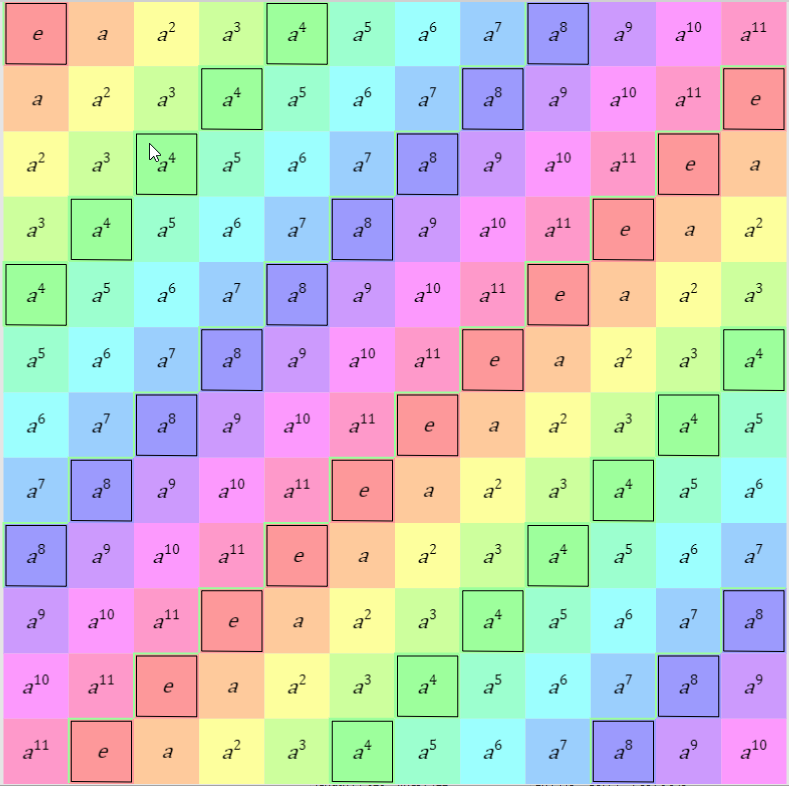
\includegraphics[scale=0.55]{images/2023-07-11_subgroup_Z12.png}
\end{figure}


\todo{show this in Gap as well}

\subsection{Subgroups generated by Subsets of a Group}

In case of cyclie subgroups, we started with one element $x$ and formed all integral powers of $x$, which amounts to closing the set $\{x\}$ under the group operation and the process of taking inverses. We now investigate the analog of this when $\{x\}$ is replaced by an arbitrary subset of $G$.


\begin{definition}
If $A$ is any subset of the group $G$ define

\bee
\langle A \rangle = \bigcap_{A \subseteq H, H \leq G} H
\eee

This is called the subgroup of $G$ generated by $A$. In other words, $\langle A \rangle$ is the intersection of all subgroups of $G$ containing $A$. If $A$ is a finite set, $A = \{a_1, a_2, \ldots, a_n \}$, then we also write $A = \langle a_1, a_2, \ldots, a_n \rangle$.
	
\end{definition}

We can show that a set defined by this definition is a subgroup of $H$, but it is a "top-down" definition and does not provide any insight into how $\langle A \rangle$ can be constructed from its elements.

A more constructive definition is

\begin{definition}
	$\langle A \rangle = \{a_1^{\epsilon_1} a_2^{\epsilon_2} \cdots a_n^{\epsilon_n} | n \in \mZ, n \geq 0, a_i \in A, \epsilon = \pm 1 \forall i  \}$
\end{definition}

In the book it is actually providen that this definition is equivalent to the more "set-centric" one above. Products of the form $a \cdot a, a \cdot a \cdot a, a \cdot a^{-1}$ etc can be simplified to $a^2, a^3, e$ etc, respectively, so another way of writing $\langle A \rangle$ is the following.

\begin{definition}
	$\langle A \rangle = \{a_1^{\alpha_1} a_2^{\alpha_2} \cdots a_n^{\alpha_n} | a_i \in A, \alpha_i \in \mZ, a_1 \neq a_{i+1}, n \in \mZ^+ \} $.
\end{definition}

In the special case $A = \{x\}$, this is the definition of $\langle x \rangle$. If $G$ is abelian, then we can commute the products around and collect all powers of a given generator $a_i$ together. If $A = \{ a_1, a_2, \ldots a_k\}$, then we would obtain

\bee
	\langle A \rangle \{ a_1^{\alpha_1} a_2^{\alpha_2} \cdots a_k^{\alpha_k} | \alpha_i \in \mZ \}
\eee

If each generator $a_i$ has a finite order $d_i$ for all $i$ and since there are exactely $d_i$ distinct powers of $a_i$, the total number of distinct products of the form $a_1^{\alpha_1} a_2^{\alpha_2} \cdots a_k^{\alpha_k}$ is at most $d_1 d_2 \cdots d_k$ and we have

\bee
	|\langle A \rangle| \leq d_1 d_2 \cdots d_k
\eee

When $G$ is non-abelian, the situation is much more complicated. For example, we cannot simplify a product $aba$ to $a^2 b$ and we therefore do not have a way to bound the group order as we were able to do when $G$ was abelian.

Asn an example consider the set $A$ containing two permutations $A = \{(1,2), (1,2,\ldots n)\}$. From \todo{where} we know that $\langle A \rangle = S_n$; therefore $S_n$ is generated by an element of order $2$ and an element of order $n$, but the order of $S_n$ is much larger, namely $n!$. 



\subsection{The Subgroup Lattice of a Group}

The subgroup lattice is a graphical representation which shows the subgroup relationship between groups. To draw the subgroup lattice of a group $G$, we start at the bottom with $\{e\}$, and end at the top with $G$. In between we place the subgroups of $G$, with subgroups of larger order positioned higher on the Figure than those of smaller order.In addition, we draw paths between two subgroups $A$ and $B$ only when $A \leq B$ and there are no subgroups properly between $A$ and $B$. Thus if $A \leq B$, there is a path (possibly many paths) upward from $A$ to $B$ passing through a chain of intermediate subgroups.

The following Figure shows the subgroup lattice for $\mZ_{12}$.

\begin{figure}[H]
\centering
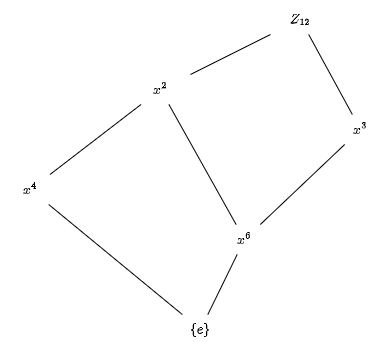
\includegraphics[scale=0.65]{images/2023-07-11_Z12_lattice.png}
\end{figure}





%%% Local Variables:
%%% mode: latex
%%% TeX-master: "journal"
%%% End:
